\documentclass[10pt,a4paper]{article}
\usepackage[utf8]{inputenc}
\usepackage{braket}
\usepackage[italian]{babel}
\usepackage{amsmath}
\usepackage{amsfonts}
\usepackage{amssymb}
\usepackage{graphicx}
\usepackage{gensymb}
\usepackage[left=2cm,right=2cm,top=2cm,bottom=2cm]{geometry}
\newcommand{\rem}[1]{[\emph{#1}]}

\author{Federico Belliardo}
\title{Tesina sulla localizzazione di Anderson: appunti}

\begin{document}
\maketitle

\section{Introduzione}
Nell'articolo 1 è riportato un esperimento in cui un condensato di Bose-Einstein viene fatto espandere in un reticolo ottico costruito sovrapponendo 2 potenziali sinusoidali (generati dalle onde stazionarie di due laser, in cui il confinamento è dato dall'effetto Stark AC) con frequenza diversa (idealmente \emph{incommensurabile}), l'ampiezza dei potenziali può essere \emph{tunata}, uno dei due ha ampiezza maggiore mentre il minore è una perturbazione.
L'articolo 2 (la prima parte) mostra come un reticolo del genere (bicromatico) sia approssimativamente equivalente a un modello detto di Aubry-Andree, a patto di translare le energie. Questo viene fatto scrivendo gli elementi di matrice dell'Hamiltoniana tra le funzioni di Wannier del reticolo principale prese gaussiane (stato fondamentale di ogni sito del reticolo) e mostrando che si possono ricondurre agli elementi di matrice del modello suddetto.\\
\section{Modello di Aubry-Andree}
L'Hamiltoniana del modello è: $\mathcal{H} = \lambda \sum_{n=0}^{N-1} cos(2 \pi \beta n) c_n ^{\dagger} c_n + t \sum_{n=0}^{N-1} (c_{n+1}^{\dagger} c_n + c_n ^{\dagger} c_{n+1})$, $\lambda$ controlla il termine di disordine e $t$ controlla quello di hopping.
Se si esegue una trasformata di fourier degli operatori, cioè: $c_n = \frac{1}{\sqrt{N}} \sum_{m=0}^{N-1} e^{i 2 \pi \beta n m} \tilde{c_m}$ si ottiene che l'Hamiltoniana si scrive come: $\mathcal{H} = 2 t \sum_{n=0}^{N-1} cos(2 \pi \beta n) \tilde{c_n}^{\dagger} \tilde{c_n} + \frac{\lambda}{2} \sum_{n=0}^{N-1} (\tilde{c_{n+1}}^{\dagger} \tilde{c_n} + \tilde{c_n}^{\dagger} \tilde{c_{n+1}})$. Questo a patto di trascurare due termini di bordo.\\
Se c'è una transizione di fase (e una sola) ci aspettiamo quindi che avvenga a $\frac{\lambda}{t} = 2$.\\
Uno stesso stato dell'Hamiltoniana può essere scritto in termini degli operatori nello spazio reale o nello spazio degli impulsi, se è "localizzato" nello spazio reale sarà delocalizzato nello spazio degli impulsi. Quello che l'articolo 3 scrive nella (1.7) è sbagliato (viene dal fatto che lui non mette radice di N nella definizione di trasformata). Tuttavia è vero che la trasformata trasforma uno stato localizzato nello spazio reale in uno esteso nello spazio degli impulsi.
$\ket{\psi} = \sum_{i=0}^{N-1} \chi_n c_n^{\dagger} \ket{\Omega} = \sum_m^{N-1} \left( \frac{1}{\sqrt{N}} \sum_{n=0}^{N-1} \chi_n e^{-i 2 \pi \beta n m} \right)\tilde{c_m}^{\dagger} \ket{\Omega}$.

Dunque uno stato localizzato, cioè i cui coefficienti sono apprezzabilmente diversi da 0 solo per un insieme limitato di siti corrisponderà ad un autostato esteso (tutti i coefficienti sono apprezzabilmente diversi da zero) per l'Hamiltoniana un cui ho eseguito la trasformazione $\frac{\lambda}{t}  \rightarrow  \frac{2}{\frac{\lambda}{t}}$. Dunque la dualità manda stati localizzati in stati estesi e viceversa.

\begin{figure}[!htb]
\centering
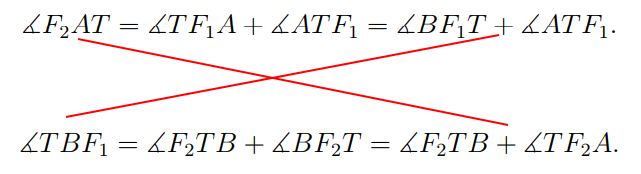
\includegraphics[scale=0.5]{immagine1.png}
\caption{Grafico della trasizione di fase.\label{fasi}}
\end{figure}

L'immagine \ref{fasi} riporta due diagrammi di fase sul carattere degli austostati al variare del rapporto $\frac{t}{\lambda}$. Di fatto non è possibile dire che vi è una sola transizione di fase (tra stati localizzati e estesi), neppure che non vi è un "mobility edge", cioè una certa energia al di sotto della quale gli stati sono localizzati e al di sopra sono estesi. Tuttavia nel limite $\frac{\lambda}{t} \rightarrow 0$ (che nella figura è chiamato $\frac{\Delta}{j}$) ho solo il termine di hopping e gli stati devono essere onde di Bloch, mentre nel limite opposto le funzioni di Wannier sono gli autostati del reticolo quindi ho localizzazione. Questa osservazione fissa anche delle condizioni su come deve essere fatto un eventuale mobility-edge (infatti sappiamo che agli estremi indipendentemente dall'energia gli autostati sono di un solo tipo).

\section{Stima della lunghezza di localizzazione - Formula di Thouless}
Nell'articolo 4 è riportata una formula per la stima della lunghezza di localizzazione degli autostati di un sistema 1D. La formula è derivata nell'ipotesi di un sistema finito e non degenere (sembra ragionevole non aspettarsi degenerazione da un modello tipo Anderson poiché non vi è nessuna sottostate simmetria) ed è estrapolata con un passaggio al continuo al caso infinito sostituendo la somma sugli stati all'integrale sulla densità degli stati \footnote{Tutti i passaggi delle derivazioni non sono riportati, ma si cerca di evidenziare  punti salienti}.\\
Si arriva a scrivere la formula: $ln | a_1^{\beta} a_N^{\beta}| = \sum_{n = 0}^{N-1} ln | V_{i, i+1} | - \sum_{\alpha \neq \beta} ln | E_{\beta} - E_{\alpha} |$. Dove $a_1^{\beta}$ e $a_N^{\beta}$ sono i coefficienti dello sviluppo dell'autostato $\beta$ sulla base di Wannier. Ora si introduce una ipotesi che credo in qualche modo giustificata a posteriori. Assumiamo una forma per i coefficienti $a_1^{\beta} = e^{-\frac{|1-i|}{\eta_{\beta}}}$ e $a_N^{\beta} = e^{-\frac{|N-i|}{\eta_{\beta}}}$, dove $i$ è la posizione del reticolo sul quale è centrato l'autostato (si cancellerà), in sostanza stiamo assumendo localizzazione per gli stati.
Da questo (e dal fatto che $V_{i, i+1} = t$), passando al continuo otteniamo una formula per la lunghezza di decadimento: $\gamma(1) = \frac{1}{\eta_{\beta}} = -\int \rho (E) ln \vert \frac{E_{beta} - E}{t} \vert dE$. Il significato della formula è che se troviamo una lunghezza reale e positiva allora il calcolo è in qualche modo autoconsistente.\\
Considerando lo stato "duale" esteso posso scrivere la sua lunghezza di correlazione come $\gamma(2) = \frac{1}{\eta_{\beta}} = -\int \rho (E) ln \vert \frac{2(E_{beta} - E)}{\lambda} \vert dE$, ma allora $\gamma(1) = \gamma(2) + ln(\frac{\lambda}{2 t})$. Se il secondo stato è esteso mi aspetto che $\gamma(2)$ sia molto piccolo e dunque $\gamma(1) = ln(\frac{\lambda}{2 t})$, cioè $l_{corr} = \frac{1}{ln(\frac{\lambda}{2 t}}$. Ci aspettiamo che la lunghezza di decadimento per uno stato localizzato sia molto piccola e la trascuriamo per ottenere una formula maneggevole.\\
La lunghezza di decadimento è disegnata sempre in figura \ref{fasi}. Si vede che vi è una sola transizione di fase, che quella lunghezza perde di senso per stati estesi (ma allora che senso aveva definirla per lo stato duale e dire che era infinita?). Vediamo anche che la lunghezza di decadimento non dipende dall'energia cioè non vi è \emph{mobility-edge}.\\


\begin{figure}[!htb]
\centering
\includegraphics[scale=0.5]{immagine6.png}
\caption{Plot del rapporto di partecipazione mediato sugli austostati.\label{partecipazione}}
\end{figure}

Si può introdurre il termine rapporto di partecipazione: $RP = \frac{\sum_{n=0}^{N-1} |a_n|^4}{\sum_{n=0}^{N-1} |a_n|^2}$, è un indice di quanto è localizzato lo stato e conferma quanto trovato precedentemente sulla lunghezza di localizzazione.

\section{Ritorno all'esperimento}
Nell'esperimento descritto nell'articolo 1 un condensato è inizialmente tenuto intrappolato in una piccola trappola armonica che viene spenta e si lascia questo evolvere sul reticolo bicromatico. 
Se gli autostati del reticolo sono onde di Bloch l'evoluzione è balistica, cioè il condensato aveva inizialmente una densità gaussiana (fondamentale della trappola) e mantiene il profilo gaussiano espandendosi cioè aumentando nel tempo la lunghezza di decadimento, finché non è diventato uniforme sul reticolo. Nella situazione in cui gli stati sono localizzati il fit del profilo di densità da invece une esponenziale decrescente (come ipotizzato nella formula di Thouless). Suppongo che queste misure vengano tutte fatte dopo un certo tempo fissato. 
Quando il condensato viene liberato la sua funzione d'onda (gaussiana) deve essere scritta in termini degli autostati del reticolo ottico e fatta evolvere, credo che intervenga il \emph{dephasing}, per cui lo stato del condensato diventa una matrice di densità sugli autostati del reticolo ottico (stato non puro) ma questo non dovrebbe essere un problema dal momento che ogni autostato ha la stessa lunghezza di decadimento prevista. Non ha modo di intervenire la termalizzazione.\\
Il meccanismo di \emph{dephasing} è quello che fa allargare la gaussiana iniziale nel caso di stati estesi. Se gli stati sono localizzati invece la funzione d'onda del condensato è somma di poche funzioni localizzate vicine. Quando interviene il \emph{dephasing} l'andamento iniziale gaussiano si trasforma in decadimento esponenziale poiché lo stato perde coerenza è si trasforma nella somma statistica delle funzioni \emph{in situ} localizzate.\\
Credo dopo un tempo fissato (cercare...) il profilo di densità è stato \emph{fittato} con una funzione del tipo $f(x) = e^{(\frac{|x-x_0|}{l})^{\alpha}}$. Il valore di $\alpha$ per varie realizzazioni del disordine è graficato in figura \ref{alpha}.

\begin{figure}[!htb]
\centering
\includegraphics[scale=0.5]{immagine2.png}
\caption{Valori del fit di $\alpha$.\label{alpha}}
\end{figure}

\begin{figure}[!htb]
\centering
\includegraphics[scale=0.5]{immagine3.png}
\caption{Larghezza "asintotica" del condensato per varie realizzazioni del disordine.\label{univ}}
\end{figure}

Il grafico \ref{univ} mostra come l'unico parametro utile per la transizione di fase sia $\frac{\lambda}{t}$.

\begin{figure}[!htb]
\centering
\includegraphics[scale=0.5]{immagine4.png}
\caption{Foto del condensato per varie realizzazioni del disordine.\label{foto}}
\end{figure}

Non ho capito benissimo ma loro sembrano assegnare un valore del parametro critico per la transizione pari a $\frac{\lambda}{t} = 6$.

\end{document}